%!TEX encoding = IsoLatin

%
% Chapitre "Cahier des charges"
%

\chapter{Cahier des charges}
\label{s:cahier_des_charges}

\section{Tableau des critères}

\begin{table}[htp]
   \footnotesize
   \centering
   \label{t:criteres}
   \begin{tabular}{|c|c|c|c|c|}
        \hline
        Critères & Pondération & Barème & Min. & Max.\\
        \hline
        \hline
        Intervention humaine & 20\% & & & \\
        \hline
        Durée de vie de la batterie [jours] & 4\% & Table \ref{t:duree_de_vie}  & 14  & \\
        Complexité de la maintenance & 4\% & Table \ref{t:bareme_complexite_maintenance} & & \\
        Automatisation du transfert de données & 6\% & Table  \ref{t:bareme_transfert_donnees} & &\\
        Accès à distance & 6\% & Table \ref{t:bareme_acces_distance} & & \\
        \hline\hline
        Qualité du produit & 40\% & & &\\
        \hline
        Durée de vie de l'appareil [années] & 4\% & Éq. \ref{eq:bareme_duree_de_vie} & &\\
        Précision du logiciel de reconnaissance [\%] & 10\% & Éq. \ref{eq:bareme_precision} & & \\
        Utilisation de l'interface graphique & 2\% & Table \ref{t:bareme_interface} & & \\
        Identification des poissons [poissons] & 10\% & Éq.  \ref{eq:bareme_identification} & 5 & \\
        Capacité de stockage des données & 7\% & Table \ref{t:bareme_stockage} & & \\
        Fiabilité du système de sécurité & 7\% & Éq. \ref{eq:bareme_sécurité} & & \\
        \hline\hline
        Coûts & 15\% & & &\\
        \hline
        Coûts de conception du produit [\$] & 4\% & Éq. \ref{eq:bareme_cout_conception} & & 10K \\
        Frais d'installation [\$] & 2\% & Éq. \ref{eq:bareme_frais_installation} & & \\
        Frais de maintenance et d'opération [\$] & 4\% & Éq. \ref{eq:bareme_frais_maintenance} & & \\
        Coûts de remplacement des pièces [\$] & 1\% & Éq. \ref{eq:bareme_cout_remplacement} & & \\
        Évaluation globale des coûts [\$] & 4\% & Table \ref{t:bareme_cout_globaux} & & 50K \\
        \hline\hline
        Facilité de conception & 10\% & & &\\
        \hline
        Temps de conception du produit [jours] & 3\% & Éq. \ref{eq:bareme_temps_conception} &  & \\
        Rechange des pièces & 3\% & Table \ref{t:bareme_difficulte_rechange} & & \\
        Complexité de l'usinage des pièces & 2\% & Table \ref{t:bareme_complexite_usinage} & & \\
        Implantation du capteur  & 2\% & Table \ref{t:bareme_implantation_capteur} & & \\
        \hline\hline
        Respect des contraintes & 15\% & & & \\
        \hline
        Prise de mesure passive & 7\% & Table \ref{t:bareme_systeme_passif} & & \\
        Contraintes mécaniques & 5\% & Table \ref{t:bareme_contraintes_mecaniques} & & \\
        Contraintes des images & 3\% & Table \ref{t:bareme_contraintes_images} & & \\
        \hline
   \end{tabular}
      \caption{Table des critères du projet Fish \& Chips}
\end{table}

\newpage{}

\section{Intervention humaine}

En analysant les demandes du client, on se rend vite compte que l’automatisation du système sera un élément prépondérant dans notre système. Pour parvenir à un système autonome, il faudra impérativement tenir compte de certains aspects comme la  durée de vie de la batterie, l’automatisation des transferts de données, l’accès à distance ainsi que la complexité de la maintenance qu’il faudra minimiser afin de réduire au maximum l’intervention humaine. Compte tenu de l’importance de cet aspect dans le projet, l’équipe de conception attribue une pondération de 20\%.

\subsection{Durée de vie de la batterie}

\begin{wraptable}{r}{5cm}
   \footnotesize
   \centering
   \scalebox{0.8}{
   \begin{tabular}{|p{3.2cm}|c|}
        \hline
        Autonomie de la batterie & Pondération\\
        \hline
        \hline
        Au moins 28 jours & 1.0 \\
        \hline
        Entre 22 et 27 jours & 0.8 \\
        \hline
        Entre 15 et 21 jours & 0.6 \\
        \hline
        Moins de 14 jours & 0.0 \\
        \hline
   \end{tabular}}
   \caption{Évaluation de la durée de vie de la batterie}
   \label{t:duree_de_vie}
\end{wraptable}

Dans l'objectif d'atteindre une autonomie minimale de deux semaines, il est nécessaire d'optimiser le système d'alimentation du capteur. De plus, afin de ne pas limiter la disponibilité du capteur, il est idéal d'utiliser une batterie à cet effet. Une batterie rechargeable permettrait également d'augmenter significativement la durée de vie du capteur optique. La durée de vie minimale demandée est de deux semaines. Le système répond entièrement au critère si celui-ci est en mesure d'accomplir deux cycles de 14 jours. De cette manière, l'opérateur possède un cycle additionnel en cas d'oubli de rechargement. L'autonomie de la batterie est évaluée selon la table \ref{t:duree_de_vie}.

\subsection{Complexité de la maintenance}

\begin{wraptable}{R}{5.5cm}
   %\footnotesize
   %\centering
   \scalebox{0.65}{
   \begin{tabular}{|c|c|}
        \hline
        Critères & Barème\\
        \hline
        \hline
        Nombre d’outils requis & \\
        \hline
        2 et moins & 1.0\\
        3 & 0.7\\
        4 & 0.4\\
        5 et plus & 0.0\\
        \hline
        \hline
        Temps nécessaire & \\
        \hline
        Moins de 30 minutes & 1.0\\
        Entre 30 et 60 minutes & 0.7\\
        Entre 60 et 120 minutes & 0.4\\
        Plus de 120 minutes & 0.0\\
        \hline
        \hline
        Fréquence d'entretien & \\
        \hline
        Une fois par année & 1.0\\
        Deux fois par an & 0.7\\
        Trois fois par an & 0.4\\
        Quatre fois ou plus par an & 0.0\\
        \hline
   \end{tabular}}
   \caption{Évaluation de la complexité de la maintenance}
   \label{t:bareme_complexite_maintenance}
\end{wraptable}

À ce sujet, il faut reconnaître que, sur le long terme, il peut y avoir des imprévus, même si tous les moyens nécessaires sont mis en œuvre pour les éviter. En cas d’imprévu, ce qui démarque un système des compétiteurs, c’est surtout comment y remédier, avec quelle facilité ou simplicité résoudre les problèmes survenus. Il s’agit là de minimiser la complexité de la maintenance en cas de pannes ou lors des entretiens. Le système le plus optimal à ce sujet est celui dont la maintenance nécessite le moins d’outils, le moins de temps et le moins d’entretien possible à long terme. Ainsi, la complexité de la maintenance comprend le nombre d'outils, le temps et la fréquence d'entretien nécessaire qui correspondent respectivement à 1\%, 1\% et 2\% du projet. Le critère présenté à la table \ref{t:bareme_complexite_maintenance} équivaut donc à une pondération totale de 4\% du projet.

%Pour évaluer les sous-critères énumérés, une note sera attribuée a chaque sous-critère et on obtient la note du concept en faisant la somme comme suit:
%  Moins d’outils (0 à 0.3) + moins de temps (0 à 0.3) + moins d’entretien (0 à 0.4) 
%Ce critère comptera par la suite pour 4\% dans le cahier des charges.

\clearpage

\subsection{Automatisation du transfert de données}

\begin{wraptable}{R}{5cm}
   %\footnotesize
   %\centering
   \scalebox{0.8}{
   \begin{tabular}{|p{3cm}|c|}
        \hline
        Transfert de données & Pondération\\
        \hline
        \hline
        Automatique et haute vitesse & 1.0 \\
        \hline
        Automatique & 0.5 \\
        \hline
        Manuel & 0.0 \\
        \hline
   \end{tabular}}
   \caption{Évaluation du barème du transfert de données}
   \label{t:bareme_transfert_donnees}
\end{wraptable}

Rappelons que dans le mandat qui a été attribué, le client attend principalement le design d’un système autonome. Cette spécification fait de l’autonomie un aspect important de notre projet. Ce qui lui a valu la pondération de 6\% dans le cahier des charges. Après la prise des images, le système doit être en mesure de les transmettre automatiquement et de les sauvegarder pour une période de deux ans au minimum sans que l'opérateur ait besoin de déplacer manuellement les données. Pour cela, on se servira d’une échelle de 0 à 1 pour évaluer à quel point nos concepts respecterons ce critère. La barème est présenté à la table \ref{t:bareme_transfert_donnees}.

\subsection{Accès à distance}

\begin{wraptable}{R}{5cm}
   \footnotesize
   \centering
   \scalebox{0.86}{
   \begin{tabular}{|c|c|}
        \hline
        Distance [m] & Barème\\
        \hline
        \hline
        X > 2000 & 1.0 \\
        \hline
        1000 < X < 2000 & 0.9 \\
        \hline
        750 < X < 1000 & 0.8 \\
        \hline
        500 < X < 750 & 0.6 \\
        \hline
        250 < X < 500 & 0.4 \\
        \hline
        100 < X < 250 & 0.2 \\
        \hline
        X < 100 & 0.0 \\
        \hline
   \end{tabular}}
   \caption{Évaluation du barème de l'accès à distance}
   \label{t:bareme_acces_distance}
\end{wraptable}

Le système que nous devons mettre en place va opérer dans un milieu où il n’est pas en contact avec l’être humain. En effet, notre système doit être capable de fonctionner à des profondeurs pouvant atteindre les 50m sous l’eau. C'est pour cette raison qu'il est important de pouvoir le contrôler à distance afin d’avoir continuellement accès au système. Ainsi, nous évaluerons ce critère à la table \ref{t:bareme_acces_distance} en utilisant le barème suivant avec X comme étant la distance qui sépare le poste de contrôle local et le système en mètres (m).

\section{Assurer la qualité de conception}

\subsection{Durée de vie de l'appareil}

La qualité supérieure du produit est un aspect déterminant du calcul de performance du design: c'est pourquoi la longévité de l'appareil entre nécessairement en ligne de compte (pondération de 4\%). La résistance de l'ensemble des composantes de la caméra se devra d'être une caractéristique à maximiser dans l'application imposée par le ministère. La résistance à la corrosion des matériaux, la contrainte de tension élastique, la tenue de vie en fatigue et la durée de vie générale des composantes électroniques incluses dans le design sont à considérer. Puisque la qualité du produit rejoint la section portant sur son autonomie, on devra porter une attention particulière à la tenue du produit à long terme: la grande durée de vie de l'appareil assure une intervention humaine minimisée. On accorde une fonction de type linéaire au barème de durée de vie de l'appareil pour assurer une valeur ajoutée constante en fonction du temps en années. Au-delà d'une période de 10 ans, on considère ce critère comme étant complètement satisfait, d'où la division par 10. Le barème prend donc la forme suivante:

\begin{equation}
    y = \frac{x}{10}
    \label{eq:bareme_duree_de_vie}
\end{equation}

\subsection{Précision du logiciel de reconnaissance}

\begin{wrapfigure}{R}{7cm}
    \centering
    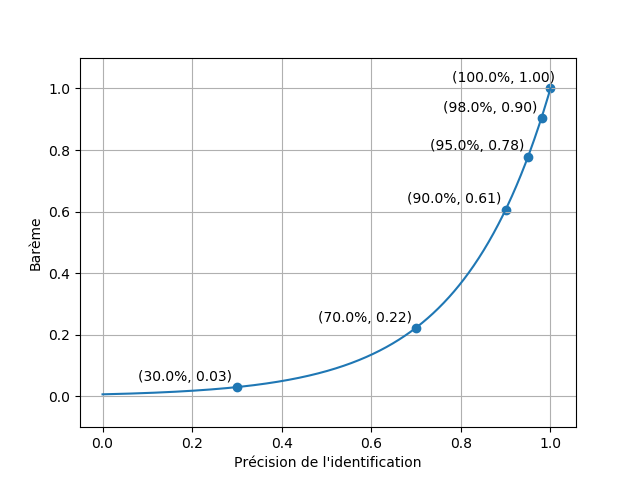
\includegraphics[width=\linewidth]{fig/bareme_ident.png}
    \caption{Illustration du barème pour la précision de l'identification des poissons}
    \label{fig:bareme_precision}
\end{wrapfigure}

Le logiciel de reconnaissance du poisson étant au coeur du projet de conception, on donnera une certaine importance à la précision et l'exactitude du programme pour assurer une collecte de données efficace (pondération de 10\%). De plus, un logiciel incapable de faire une bonne différenciation des espèces de poissons ruine l'ensemble des investissements ultérieurs: une excellente caméra ne vaut rien sans un logiciel de qualité. Par contre, à une différenciation d'exactitude dans les très hauts pourcentages (85 à 100), on donnera graduellement moins d'importance aux variations d'efficacité. À un tel niveau d'exactitude, on laissera plus d'importance aux autres caractéristiques en considérant la précision de l'appareil déjà pratiquement maximisée. La fonction quantifiant la qualité de la reconnaissance du poisson s'apparente à une fonction de type racine carrée tel que présenté ci-contre:

\begin{equation}
    y = e^{5(x-1)}
    \label{eq:bareme_precision}
\end{equation}

\subsection{Utilisation de l'interface graphique}

\begin{wraptable}{R}{7cm}
   \footnotesize
   \centering
   \scalebox{0.8}{
   \begin{tabular}{|c|c|}
        \hline
        Difficulté de l'utilisation de l'interface & Barème \\
        \hline
        \hline
        Très facile & 1.0 \\
        \hline
        Facile & 0.8 \\
        \hline
        Intermédiaire & 0.6 \\
        \hline
        Difficile & 0.4 \\
        \hline
        Très difficile & 0.0 \\
        \hline
   \end{tabular}}
   \caption{Évaluation du barème de l'interface graphique}
   \label{t:bareme_interface}
\end{wraptable}

Puisque l'optique principale de ce projet tourne autour une automatisation des tâches, l'aisance d'utilisation de l'interface lors de l'accès aux données et des opérations de maintenance bimensuelles rejoint tout autant la ligne directrice du design d'appareil (pondération de 2\%). La différenciation entre un interface graphique excellent et médiocre étant difficile à quantifier par calcul, on donnera un barème sous forme de charte, où la valeur la plus grande sera accordée à une qualification de "très intuitive" et la plus faible à "très difficile d'utilisation". La charte des barèmes est présentée à la table \ref{t:bareme_interface}. 

\subsection{Identification des poissons}

\begin{wrapfigure}{R}{6.5cm}
    \centering
    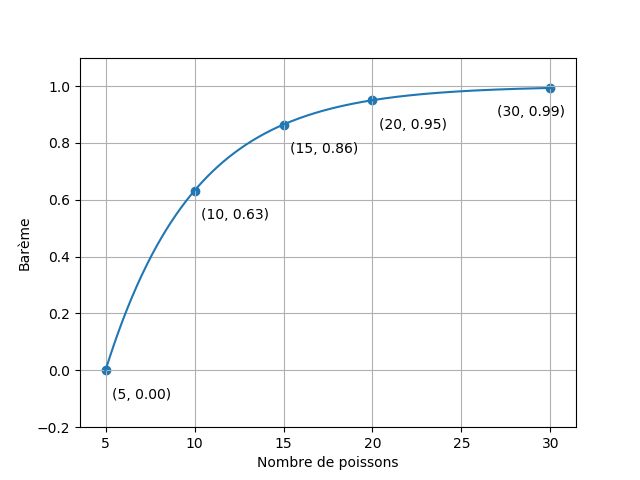
\includegraphics[width=\linewidth]{fig/bareme_identification.png}
    \caption{Barème pour le nombre de poissons à identifier}
    \label{fig:bareme_identification}
\end{wrapfigure}

La quantité de poissons reste également à considérer dans l'implantation du système dans la mesure où deux sites différents peuvent chacun comporter une faune aquatique distinctive. Une optimisation de la taille de la librairie des poissons est d'une grande importance lors de la collecte des données par l'appareil: ce dernier doit évidemment être en mesure d'effectuer une bonne reconnaissance du type de poisson. On donnera donc à cette session une pondération de 10\%. Une variété de poisson trop stricte de la librairie causerait une collecte de données erronées dans certain milieux. Il est aussi à noter que le nombre de poissons à considérer est de cinq par site. On définira une équation exponentielle pour la gradation de ce barème: la clé du succès de ce critère repose dans la maximisation du nombre de poisson reconnaissables par la caméra. Par contre, on accordera graduellement moins d'importance à ce critère si le logiciel accepte déjà une grande quantité d'espèces marines. Avec un tel barème, on peut ainsi assurer la compatibilité du logiciel pour son implantation dans différents sites où la faune aquatique pourrait varier.

\begin{equation}
    y = -e^{-0.2(x-5)} + 1
    \label{eq:bareme_identification}
\end{equation}


\subsection{Capacité de stockage des données}

\begin{wraptable}{R}{6.5cm}
   %\footnotesize
   %\centering
   \begin{tabular}{|p{4cm}|c|}
        \hline
        Capacité de stockage des données & Barème\\
        \hline
        Répond aux critère & 1 \\
        \hline
        Ne répond pas aux critère & 0 \\
        \hline
   \end{tabular}
   \caption{Évaluation du barème du stockage de données}
   \label{t:bareme_stockage}
\end{wraptable}

La collecte de données est un aspect primordial dans l'énonciation des critères imposés par le ministère: il est impératif que la taille de stockage puisse accepter des données allant jusqu'à une période de deux ans, et ce, à des fins de vérification. Il est à souligner ici qu'il n'y a aucun avantage à stocker les données pendant une période plus importante que celle imposée par le ministère: c'est pourquoi un barème de type binaire est le plus approprié ici. On affectera la valeur 1 au critère si le système de stockage de données répond bien au besoins du client, et 0 si le critère n'est pas satisfait (Table \ref{t:bareme_stockage}).

\subsection{Fiabilité du système de sécurité}

%\begin{wrapfigure}{R}{6cm}
%    \centering
%    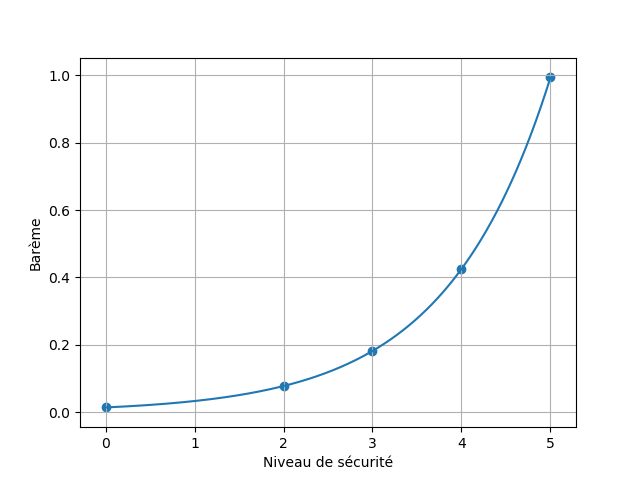
\includegraphics[width=\linewidth]{fig/Securite.png}
%    \caption{Illustration du barème du système de sécurité}
%    \label{fig:bareme_securite}
%\end{wrapfigure}

La confidentialité et l'authenticité des données est primordiale dans un tel projet: c'est pourquoi une grande partie de la cote associée à la qualité du design dépendra de la sécurité du produit. C'est pourquoi un 7\% de la note sera accordée à la sécurité. Plusieurs protocoles de conservation et de transfert des données devront être mis en place, et ce seront justement ici le nombre et la qualité des couches de sécurité offertes par le produit qui permettront une véritable quantification de ce critère. Puisque le système à livrer est fortement axé sur l'autonomie et l'accès à distance, un système qui est facilement compromis est à proscrire à tout prix. Une fonction exponentielle représente parfaitement l'enjeu ici: la moindre faiblesse du système de sécurité peut rendre le produit complètement inutilisable. Le niveau de sécurité $x$ est une combinaison du nombre de couches de sécurité pondéré par leurs qualités respectives.

\begin{equation}
    y = 0.849 e^{0.014x}
    \label{eq:bareme_sécurité}
\end{equation}

\section{Coûts}
Une limite des coûts a été établie : on ne peut dépasser 10 000 dollars de frais matériel et 40 000 dollars de coûts humains. Ainsi, ces deux éléments sont à traiter indépendamment l’un de l’autre mais on peut considérer l’importance d’un coût global de 50 000 dollars. De ce fait, on considère une proportion égale de ces deux sources de dépense lors de l’évaluation globale des coûts afin de simplifier l’analyse et la compréhension des coûts liés à la fabrication et à l’entretien de la machine. Cependant, un budget attitré sera alloué à chacune de ses sections pour chaque source de dépense spécifique, et seront considérés séparément au moment de l’analyse des coûts du produit.

\subsection{Coûts de conception du produit}
La première étape précédant l’utilisation de la machine, est sa conception. Cette partie est non négligeable dans le processus d’analyse des coûts de la machine car elle représente la plus grande source de dépense en matériaux. Afin de combler les besoins du Ministère, on cherche à minimiser les coûts totaux liés à la fabrication de la machine. Toutefois, en adoptant un budget minimal pour fabriquer le système, les composants choisis ne seront pas les plus performants. De plus, cette machine doit être le plus autonome possible et doit donc nécessiter le moins de maintenance possible. On a donc un certain avantage à dépenser un peu plus que le minimum, pour obtenir une machine qui dure plus longtemps sans intervention. En parallèle, il faut limiter les coûts pour que le Ministère puisse économiser et favorisera ainsi le projet.
Ainsi, la fonction décrivant l’efficacité par rapport au coût de production suit une forme suivante :

\begin{equation}
    E(S) = \frac{-(S-10000)^2+100000}{100000000} + 1
    \label{eq:bareme_cout_conception}
\end{equation}

Ici $S$ représente le montant en dollars canadiens investis à partir du budget matériel en $S$ varie entre 0 et 10 000. $E$ représente l’efficacité notée sur 1. Le budget matériel est au maximum de 10 000 dollars. Considérant l'importance du respect des coûts de conception, une pondération de 4\% a donc été attribué à ce critère.


\subsection{Frais d'installation}
Ici, il est certain que chercher à dépenser pour l’installation est futile. En effet, on ne cherche qu’à placer la machine là où les mesures seront faites. Ainsi, si on ne dépense que le strict minimum sur l’installation, on pourra avoir un budget optimal sans se limiter sur un autre aspect du projet. Pour les frais d'installation, on a attribué une pondération de 2\% de l'ensemble du projet. 
On peut représenter cette composante des frais sous la forme :

\begin{equation}
E(S) = \frac{10}{S+10}
\label{eq:bareme_frais_installation}
\end{equation}

\subsection{Frais de maintenance et d'opération}
En ce qui concerne les frais de maintenance et d’opérations, on se retrouve face à un dilemme similaire à celui du coût de constructions. En effet, si on investi trop peu d’argent, la machine se brisera plus rapidement et il faudra débourser encore plus dans la machine. Cependant, on cherche à limiter l’argent mis dans le projet pour ne pas trop alléger le portefeuille du ministère.
Ainsi, on retrouve une fonction telle que :

\begin{equation}
    E(S) = \frac{−(S−20000)^2+ 100000000}{100000000}
    \label{eq:bareme_frais_maintenance}
\end{equation}

Ici, tel que précédemment, on doit dépenser un certain montant pour s’assurer du fonctionnement du procédé de collecte de données et de l’entretien, si on en a le besoin. De ce fait, on cherche à ne pas dépasser 2000 dollars d’investissement mais viser à dépenser moins ne serait pas une décision des plus sages. Également on paye pour les employés qui seront formés et travailleront auprès du robot. Les frais de maintenance et d'opération représente 4\% du projet.

\subsection{Coûts de remplacement des pièces}
Enfin, s’il est nécessaire de racheter certaines pièces, il faut considérer s’il ne serait pas préférable de ne pas remplacer complètement la machine. Si les coûts arrivent proches de celui d’une nouvelle machine, il sera alors préférable d’en racheter une nouvelle car elle aura une meilleure durée de vie dans tous les cas. À partir de 20 000 dollars de réparation, il est impératif de changer de robot. Donc, l’efficacité en fonction du prix suit une courbe linéaire de type :
\begin{equation}
    E(S) = 1-0.0005\cdot S
\label{eq:bareme_cout_remplacement}
\end{equation}

\subsection{Évaluation globale des coûts}

\begin{wraptable}{R}{5cm}
   %\footnotesize
   %\centering
   \scalebox{0.9}{
   \begin{tabular}{|c|c|}
  \hline
  Prix & Barème\\
  \hline
  Dntre 0\$ à 20 000\$ & 1.0 \\
  \hline
  De 20 000\$ à 35 000\$ & 0.7 \\
  \hline
  De 35 000\$ à 50 000\$ & 0.4 \\
  \hline
  Supérieur à 50 000\$ & 0.0 \\
  \hline
\end{tabular}}
\caption{Évaluation du barème des coûts globaux}
\label{t:bareme_cout_globaux}
\end{wraptable}

Considérant l'importance de respecter les coûts de conception et de main-d'oeuvres, l'évaluation globale des coûts possède une pondération de 4\%. En effet, tel que demandé par le client, les frais de main-d'oeuvres ne doivent pas dépasser les 40 000\$ alors que les frais de conception ne doivent pas dépasser 10 000\$. En somme, les coûts globaux ne doivent pas atteindre plus que 50 000\$ sans quoi la solution sera systématiquement rejetée. Le barème est défini à la table \ref{t:bareme_cout_globaux}.

\section{Facilité de conception}

\subsection{Temps de conception du produit}

Le temps de conception du produit doit être minimisé pour des raisons pratiques et financières: si le produit prend peu de temps à concevoir, il pourra être déployé plus rapidement et les coûts de conception en temps de personnel seront diminués. La formule utilisée pour le barème est la suivante:

\begin{equation}
    y=e^{-0.14t}
\label{eq:bareme_temps_conception}    
\end{equation}

où le temps est exprimé en jours.

%\begin{figure}[htb]
%    \centering
%    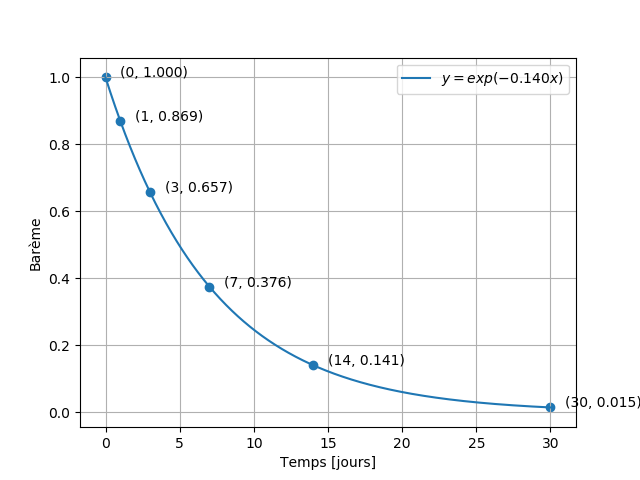
\includegraphics[width=0.45\linewidth]{fig/Temps_de_conception.png}
%    \caption{Illustration du barème du temps de conception}
%    \label{fig:temps_de_conception_bareme}
%\end{figure}

\subsection{Rechange des pièces}

\begin{wraptable}{R}{5cm}
   %\footnotesize
   %\centering
   \scalebox{0.7}{
   \begin{tabular}{|p{3cm}|c|}
        \hline
        Difficulté de la rechange des pièces & Barème\\
        \hline
        \hline
        Très facile & 1.00 \\
        \hline
        Facile & 0.75 \\
        \hline
        Difficile & 0.50 \\
        \hline
        Très difficile & 0.25 \\
        \hline
        Impossible & 0.00 \\
        \hline
   \end{tabular}}
   \caption{Évaluation du barème de la difficulté de la rechange des pièces}
   \label{t:bareme_difficulte_rechange}
\end{wraptable}

Bien que toutes les mesures seront prises pour que ça n'arrive pas, il se pourrait qu'il y ait un bris quelconque dans le système. Le produit doit donc être bien conçu pour que la rechange des pièces soit facile. Une rechange des pièces qualifiée de «très facile» pourrait être fait par n'importe qui, et ce, même si la personne en charge n'est pas manuelle. Une rechange des pièces qui est «difficile» est tout de même préférable, puisqu'au moins il est possible de changer les pièces. Le pire des cas serait une rechange «impossible» où il faudrait changer tout le système s'il y a un bris quelconque, même dans un dispositif anodin. Le barème est présenté à la table \ref{t:bareme_difficulte_rechange}.

\subsection{Complexité de l'usinage des pièces}

\begin{wraptable}{R}{5cm}
   \scalebox{0.52}{
   \begin{tabular}{|c|c|}
        \hline
        Complexité de l'usinage des pièces & Barème\\
        \hline
        \hline
        Très peu complexe & 1.00 \\
        \hline
        Peu complexe & 0.75 \\
        \hline
        Neutre & 0.50 \\
        \hline
        Complexe & 0.25 \\
        \hline
        Très complexe & 0.00 \\
        \hline
   \end{tabular}}
   \caption{Barème de la complexité de l'usinage des pièces}
   \label{t:bareme_complexite_usinage}
\end{wraptable}

À toutes fins pratiques, le projet tire avantage à ce que l'usinage des pièces soit le moins complexe possible. Des pièces plus faciles à usiner feront diminuer le temps lié à la conception du produit et aussi aux dépenses reliées à l'équipement requis pour la conception. Dans une optique où le coût du projet doit être minimisé, il est nécessaire de prendre en compte la complexité de l'usinage des pièces. Le barème est présenté à la table \ref{t:bareme_complexite_usinage}. Un usinage dit «très peu complexe» correspond à un usinage ou un assemblage qui pourrait entièrement se faire avec des outils de base. On pense par exemple à un atelier dans une maison. Un usinage «peu complexe» à «complexe» pourrait se réaliser avec l'aide d'outils plus spécialisés, dépendemment du nombre d'outils spécialisés. Un usinage «très complexe» serait fait avec l'aide d'un machiniste ou un autre spécialiste qui devrait travailler plusieurs pièces afin de les assembler.


\subsection{Implantation du capteur}

\begin{wraptable}{R}{6cm}
   %\footnotesize
   %\centering
   \scalebox{0.7}{
   \begin{tabular}{|c|c|}
        \hline
        Facilité de l'implantation du capteur & Barème\\
        \hline
        \hline
        Très peu complexe & 1.00 \\
        \hline
        Peu complexe & 0.75 \\
        \hline
        Neutre & 0.50 \\
        \hline
        Complexe & 0.25 \\
        \hline
        Très complexe & 0.00 \\
        \hline
   \end{tabular}}
   \caption{Évaluation du barème de la facilité de l'implantation du capteur}
   \label{t:bareme_implantation_capteur}
\end{wraptable}

Puisque le client souhaite implanter le capteur sur plusieurs sites pour acquérir des données, on considère qu'il serait préférable que l'installation du capteur soit facile. C'est aussi avantageux d'un point de vue économique puisque cela pourrait potentiellement réduire les frais d'installation. Étant donné c'est le client qui se charge d'implanter et d'installer le capteur sur les sites, il est de notre devoir de lui faciliter la tâche pour lui donner un meilleur service. Une implantation «très peu complexe» pourrait être faite par un employé non spécialisé. À l'opposé, une implantation «très complexe»  pourrait seulement être faite par un technicien qui connaît bien le produit. Le barème est montré à la table \ref{t:bareme_implantation_capteur}.

\section{Respect des contraintes}

\subsection{Prise de mesure passive}

Bien que l'objectif principal du capteur est d'identifier une variété de poissons dans un milieu aquatique, il est nécessaire que cette identification n'affecte pas le mode de vie des poissons. En effet, l'une des principales motivations du client à l'égard du projet Fish \& Chips est d'assurer une mesure passive. Le capteur optique ne doit en aucun cas perturber l'environnement des poissons évoluant sur le site. Une importance relative de 7\% est donc accordé à ce critère. En cas de perturbation de l'environnement, le design est automatiquement rejeté, comme le précise la table \ref{t:bareme_systeme_passif}. 

\begin{table}[htp]
   \footnotesize
   \centering
   \begin{tabular}{|c|c|}
        \hline
        Degré de passivité du système & Barème\\
        \hline
        \hline
        Le système assure une mesure passive & 1.0 \\
        \hline
        Le système n'assure pas une mesure passive & 0.0 \\
        \hline
   \end{tabular}
   \caption{Évaluation du barème du degré de passivité du système}
   \label{t:bareme_systeme_passif}
\end{table}

\subsection{Contraintes mécaniques}

Le capteur optique doit respecter certaines contraintes physiques et mécaniques. Le non respect de ces contraintes ne doit en aucun cas affecter les fonctionnalités du système. De plus, l'aspect physique du capteur optique ne doit pas être un facteur pouvant perturber l'environnement des poissons. C'est dans cette optique qu'on attribue aux contraintes mécaniques une pondération de 5\% de l'ensemble du projet. Ce barème a été calculé considérant le tableau \ref{t:bareme_contraintes_mecaniques} et les caractéristiques suivantes:

Le capteur optique doit posséder une masse inférieure à 5kg sous l'eau. Le volume du capteur sous l'eau se doit de ne pas dépasser 0.3$m^{3}$. Le capteur doit être fonctionnel jusqu'à une profondeur de 50 pieds. Le système doit supporter une température entre +5°C et -10°C par rapport à la température de l'eau où le capteur sera situé.

%\begin{enumerate}
%    \item Le capteur optique doit posséder une masse inférieure à 5kg sous l'eau.
%    \item Le volume du capteur sous l'eau se doit de ne pas dépasser 0.3$m^{3}$. 
%    \item Le capteur doit être fonctionnel jusqu'à une profondeur de 50 pieds.
%    \item Le système doit supporter une température entre +5°C et -10°C par rapport à la température de l'eau où le capteur sera situé.
%\end{enumerate}

\begin{table}[htb!]
   \footnotesize
   \centering
   \begin{tabular}{|c|c|}
        \hline
        Caractéristiques mécaniques respectées & Barème\\
        \hline
        \hline
        Le système respecte l'ensemble des caractéristiques & 1.0 \\
        \hline
        Le système ne respecte pas l'une des caractéristiques & 0.0 \\
        \hline
   \end{tabular}
   \caption{Évaluation des contraintes mécaniques du système}
   \label{t:bareme_contraintes_mecaniques}
\end{table}

\subsection{Contraintes des images}

En plus reconnaître et de comptabiliser des espèces de poissons, le système doit être en mesure de prendre une image du poisson identifié à des fins de validation. Ces images comprennent quelques caractéristiques a respecter tel que demandé par le Ministère de la Faune Aquatique. La qualité des images est nécessaire afin de maximiser la précision de l'identification des poissons. La pondération de ce critère est mesurée à l'aide du tableau \ref{t:bareme_contraintes_images} et des caractéristiques suivantes:

Les images capturées doivent être en couleur. La taille des images ne doit pas excéder 8 bits. Les dimensions des photos doivent être de 100 X 100 pixels. Chacune des images recueillies doivent également fournir la date et l'heure, la température interne du système, la température de l'eau et l'identification du poisson. Le capteur optique doit être en mesure d'observer des spécimens de plus de 6cm. Le système doit être en mesure de capter des poissons dans un volume minimal de 1$m^{3}$.


%   \begin{enumerate}
%       \item Les images capturées doivent être en couleur.
%       \item La taille des images ne doit pas excéder 8 bits.
%       \item Les dimensions des photos doivent être de 100 X 100 pixels.
%       \item Chacune des images recueillies doivent également fournir la date et l'heure, la           température interne du système, la température de l'eau et l'identification du poisson.
%       \item Le capteur optique doit être en mesure d'observer des spécimens de plus de 6cm.
%       \item Le système doit être en mesure de capter des poissons dans un volume minimal de           1$m^{3}$.
%    \end{enumerate}

Considérant l'ensemble de ces caractéristiques, on a accordé une pondération de 3\% pour les contraintes des images.

\begin{table}[htp]
   \footnotesize
   \centering
   \begin{tabular}{|c|c|}
        \hline
        Caractéristiques des images respectées & Barème\\
        \hline
        \hline
        Le système respecte l'ensemble des caractéristiques & 1.0 \\
        \hline
        Le système ne respecte pas l'une des caractéristiques & 0.0 \\
        \hline
   \end{tabular}
   \caption{Évaluation des contraintes reliées aux images}
   \label{t:bareme_contraintes_images}
\end{table}

\newpage


\section{Maison de qualité}

\begin{figure}[htb!]
    \centering
    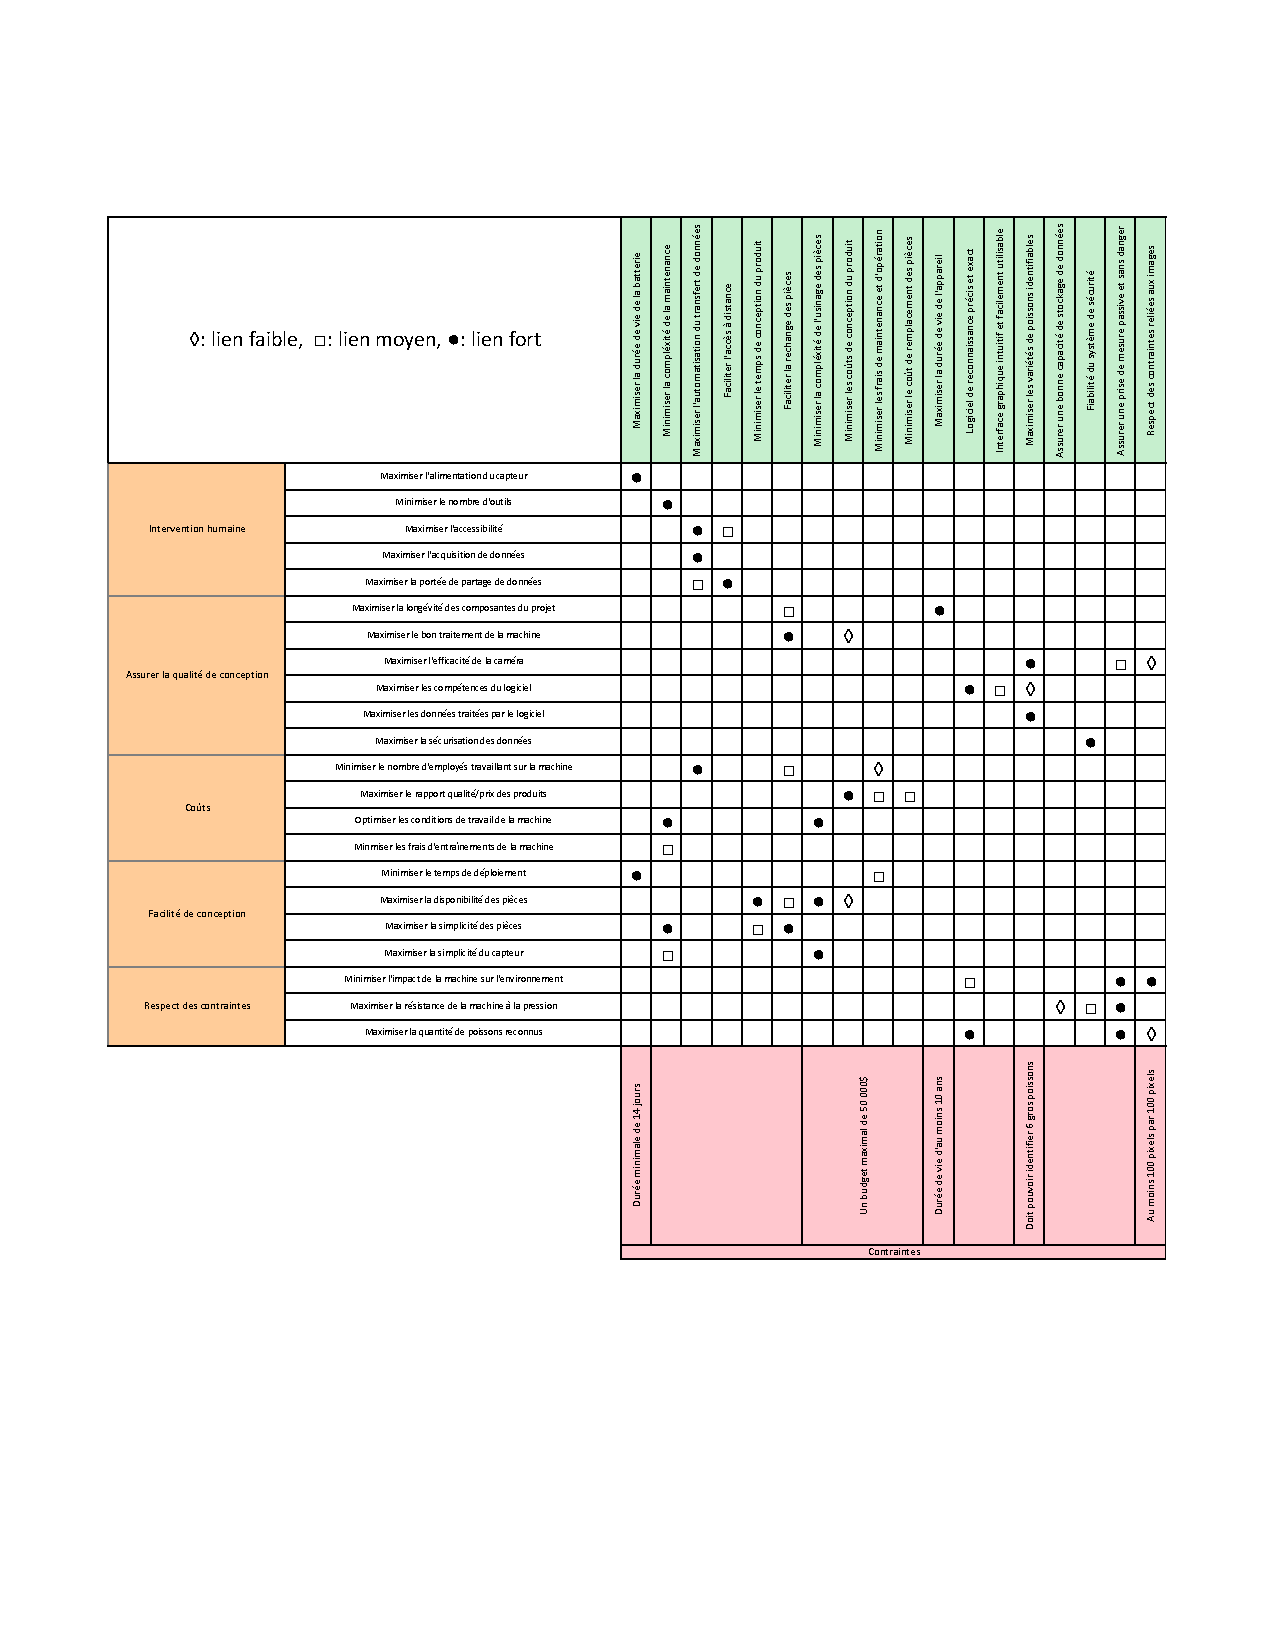
\includegraphics[width=0.90\linewidth]{fig/maison_de_qualite.pdf}
    \caption{Maison de qualité du projet Fish \& Chips}
    \label{fig:maison_qualite}
\end{figure}




